% 2004 年春季安徽文科卷第 20 题：三棱柱示意图；not to scale.
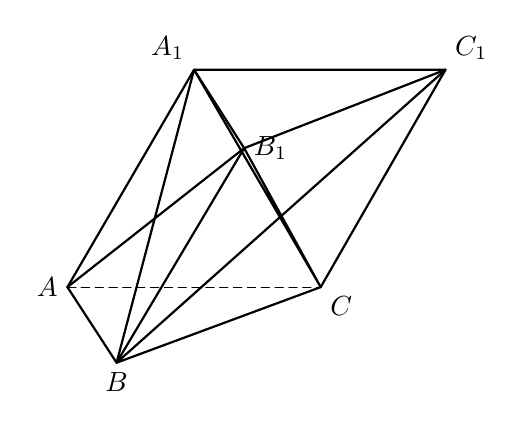
\begin{tikzpicture}[line cap=round,line join=round,scale=1.2]
  \coordinate (A) at (0,0);
  \coordinate (B) at (0.52,-0.80);
  \coordinate (C) at (2.68,0);
  \coordinate (A1) at (1.34,2.30);
  \coordinate (B1) at (1.87,1.47);
  \coordinate (C1) at (4.00,2.30);

  % Hidden base edge in the source drawing.
  \draw[densely dashed] (A) -- (C);
  % Triangular bases and corresponding lateral edges.
  \draw[thick] (A) -- (B) -- (C);
  \draw[thick] (A1) -- (B1) -- (C1) -- cycle;
  \draw[thick] (A) -- (A1) (B) -- (B1) (C) -- (C1);
  % Construction lines shown in the source figure for the two subquestions.
  \draw[thick] (A1) -- (B) (A1) -- (C) (A) -- (B1) (B1) -- (C) (B) -- (C1);

  \node[left] at (A) {$A$};
  \node[below] at (B) {$B$};
  \node[below right] at (C) {$C$};
  \node[above left] at (A1) {$A_1$};
  \node[right] at (B1) {$B_1$};
  \node[above right] at (C1) {$C_1$};
\end{tikzpicture}
